\documentclass[a4paper,12pt]{article}

% Setting up the preamble
\usepackage[utf8]{inputenc}
\usepackage[T1]{fontenc}
\usepackage{geometry}
\geometry{margin=1in}
\usepackage{listings}
\usepackage{xcolor}
\usepackage{fancyhdr}
\usepackage{graphicx} % For including images
\usepackage{float}
\usepackage{tocloft}
\usepackage{parskip}

% Configuring listings for code display (matching page 10)
\lstset{
    basicstyle=\ttfamily\small,
    breaklines=true,
    frame=single,
    numbers=none,
    keywordstyle=\color{blue},
    commentstyle=\color{gray},
    stringstyle=\color{red},
    showstringspaces=false,
    tabsize=2,
}

% Configuring header and footer (empty)
\pagestyle{empty}
\fancyhf{}

% Setting up font
\usepackage{noto}

% Document title and author
\title{BCA 3rd Semester Web Technology Lab Report}
\author{ Anupam Baral}
\date{ 2025}

\clearpage

\begin{document}

\maketitle
\tableofcontents
\newpage

\section{Introduction}
This lab report implements a student registration system using HTML, CSS, PHP, and MySQL, with XML for structured data. It includes a registration form, a student information table, CRUD operations, and XML examples for student and employee data. Output images are included to demonstrate the rendered results. All code listings are formatted consistently with a monospaced font, small size, and single-line spacing.

\section{Student Registration Form}
The form collects roll number, personal details, faculty, subjects, photo, and comments, styled with CSS and validated with JavaScript.

\lstset{language=HTML}
\begin{lstlisting}
<!DOCTYPE html>
<html lang="en">
<head>
  <title>Student Registration Form</title>
  <meta charset="UTF-8">
  <meta name="viewport" content="width=device-width, initial-scale=1.0">
  <style>
    * {
      margin: 0;
      padding: 0;
      box-sizing: border-box;
    }
    body {
      font-family: 'Segoe UI', Tahoma, Geneva, Verdana, sans-serif;
      background: linear-gradient(135deg, #667eea 0%, #764ba2 100%);
      min-height: 100vh;
      padding: 20px;
    }
    .container {
      max-width: 800px;
      margin: 0 auto;
      background: white;
      border-radius: 15px;
      box-shadow: 0 20px 40px rgba(0, 0, 0, 0.1);
      overflow: hidden;
    }
    .header {
      background: linear-gradient(135deg, #4facfe 0%, #00f2fe 100%);
      color: white;
      text-align: center;
      padding: 30px;
    }
    .header h1 {
      font-size: 2rem;
      margin-bottom: 10px;
    }
    .form-container {
      padding: 40px;
    }
    .form-row {
      display: flex;
      margin-bottom: 25px;
      align-items: flex-start;
      gap: 20px;
    }
    .form-row label {
      flex: 0 0 200px;
      font-weight: 600;
      color: #333;
      padding-top: 8px;
    }
    input[type="text"],
    input[type="number"],
    input[type="tel"],
    input[type="date"],
    input[type="file"],
    select,
    textarea {
      width: 100%;
      padding: 12px 15px;
      border: 2px solid #e1e5e9;
      border-radius: 8px;
      font-size: 14px;
      transition: all 0.3s ease;
      font-family: inherit;
    }
    .radio-item,
    .checkbox-item {
      display: flex;
      align-items: center;
      gap: 8px;
    }
    input[type="radio"],
    input[type="checkbox"] {
      width: auto;
      margin: 0;
      transform: scale(1.2);
    }
    textarea {
      resize: vertical;
      min-height: 100px;
    }
    .button-group {
      display: flex;
      gap: 15px;
      justify-content: center;
      margin-top: 30px;
    }
    .btn {
      padding: 12px 30px;
      border: none;
      border-radius: 8px;
      font-size: 16px;
      font-weight: 600;
      cursor: pointer;
      transition: all 0.3s ease;
      text-transform: uppercase;
      letter-spacing: 0.5px;
    }
    .btn-primary {
      background-color: #4facfe;
      color: white;
    }
    .btn-secondary {
      background-color: #ccc;
      color: #333;
    }
  </style>
</head>
<body>
  <div class="container">
    <div class="header">
      <h1>Student Registration</h1>
      <p>Please fill out all required information</p>
    </div>
    <div class="form-container">
      <form id="studentForm">
        <div class="form-row">
          <label for="rollNo">Roll Number</label>
          <div class="input-group">
            <input type="number" id="rollNo" name="rollNo" placeholder="Enter your roll number" required>
          </div>
        </div>
        <div class="form-row">
          <label for="fullName">Full Name</label>
          <div class="input-group">
            <input type="text" id="fullName" name="fullName" placeholder="Enter student's full name" required>
          </div>
        </div>
        <div class="form-row">
          <label for="address">Address</label>
          <div class="input-group">
            <input type="text" id="address" name="address" placeholder="Enter student's address" required>
          </div>
        </div>
        <div class="form-row">
          <label for="phone">Phone Number</label>
          <div class="input-group">
            <input type="tel" id="phone" name="phone" placeholder="Enter phone number" required>
          </div>
        </div>
        <div class="form-row">
          <label>Gender</label>
          <div class="input-group">
            <div class="radio-group">
              <div class="radio-item">
                <input type="radio" id="male" name="gender" value="male" required>
                <label for="male">Male</label>
              </div>
              <div class="radio-item">
                <input type="radio" id="female" name="gender" value="female" required>
                <label for="female">Female</label>
              </div>
              <div class="radio-item">
                <input type="radio" id="other" name="gender" value="other" required>
                <label for="other">Other</label>
              </div>
            </div>
          </div>
        </div>
        <div class="form-row">
          <label for="dob">Date of Birth</label>
          <div class="input-group">
            <input type="date" id="dob" name="dob" required>
          </div>
        </div>
        <div class="form-row">
          <label>Subjects of Interest</label>
          <div class="input-group">
            <div class="checkbox-group">
              <div class="checkbox-item">
                <input type="checkbox" id="ai" name="subjects" value="ai">
                <label for="ai">Artificial Intelligence</label>
              </div>
              <div class="checkbox-item">
                <input type="checkbox" id="dba" name="subjects" value="dba">
                <label for="dba">Database Administration</label>
              </div>
              <div class="checkbox-item">
                <input type="checkbox" id="nsa" name="subjects" value="nsa">
                <label for="nsa">Network Security</label>
              </div>
            </div>
          </div>
        </div>
        <div class="form-row">
          <label for="faculty">Select Faculty</label>
          <div class="input-group">
            <select id="faculty" name="faculty" required>
              <option value="">-- Select Faculty --</option>
              <option value="bca">Bachelor of Computer Application (BCA)</option>
              <option value="bba">Bachelor of Business Administration (BBA)</option>
              <option value="bbs">Bachelor of Business Studies (BBS)</option>
            </select>
          </div>
        </div>
        <div class="form-row">
          <label for="photo">Upload Photo</label>
          <div class="input-group">
            <input type="file" id="photo" name="photo" accept="image/*">
          </div>
        </div>
        <div class="form-row full-width">
          <label for="comments">Additional Comments</label>
          <div class="input-group">
            <textarea id="comments" name="comments" placeholder="Write any additional information or comments here..."></textarea>
          </div>
        </div>
        <div class="button-group">
          <button type="submit" class="btn btn-primary">Submit Application</button>
          <button type="reset" class="btn btn-secondary">Reset Form</button>
        </div>
      </form>
    </div>
  </div>
  <script>
    document.getElementById('studentForm').addEventListener('submit', function(e) {
      e.preventDefault();
      alert('Form submitted successfully! (This is a demo)');
    });
    document.querySelector('.btn-secondary').addEventListener('click', function() {
      if (confirm('Are you sure you want to reset the form?')) {
        document.getElementById('studentForm').reset();
      }
    });
  </script>
</body>
</html>
\end{lstlisting}

\subsection{Form Output}
The rendered output of the student registration form is shown below.

\begin{figure}[h]
    \centering
    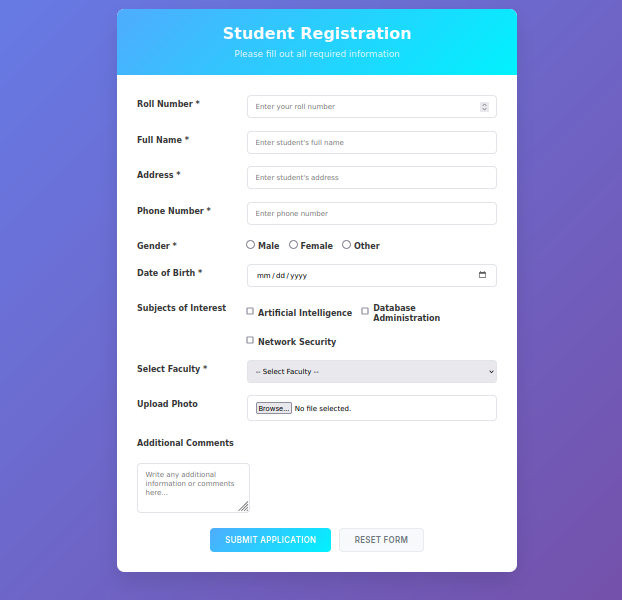
\includegraphics[width=0.8\textwidth]{10_screenshot.png}
    \caption{Student Registration Form Output}
\end{figure}

\section{Student Information Table}
The table displays student data with CSS styling for a clean look.

\lstset{language=HTML}
\begin{lstlisting}
<!DOCTYPE html>
<html lang="en">
<head>
  <meta charset="UTF-8">
  <meta name="viewport" content="width=device-width, initial-scale=1.0">
  <title>Student Information Table</title>
  <style>
    body {
      font-family: Arial, sans-serif;
      margin: 20px;
      background-color: #f5f5f5;
    }
    .container {
      max-width: 1000px;
      margin: 0 auto;
      background-color: white;
      padding: 30px;
      border-radius: 8px;
      box-shadow: 0 2px 10px rgba(0, 0, 0, 0.1);
    }
    h1 {
      text-align: center;
      color: #333;
      margin-bottom: 30px;
    }
    table {
      width: 100%;
      border-collapse: collapse;
      margin: 20px 0;
      font-size: 16px;
    }
    th {
      background-color: #4CAF50;
      color: white;
      padding: 12px 15px;
      text-align: left;
      font-weight: bold;
    }
    td {
      padding: 12px 15px;
      text-align: left;
      border-bottom: 1px solid #ddd;
    }
    .table-info {
      text-align: center;
      margin-bottom: 20px;
      color: #666;
      font-style: italic;
    }
  </style>
</head>
<body>
  <div class="container">
    <h1>Student Information Database</h1>
    <p class="table-info">Complete list of registered students for Academic Year 2024-25</p>
    <table>
      <thead>
        <tr>
          <th>Roll No</th>
          <th>Student Name</th>
          <th>Age</th>
          <th>Gender</th>
          <th>Faculty</th>
          <th>Email</th>
          <th>Phone Number</th>
          <th>City</th>
        </tr>
      </thead>
      <tbody>
        <tr>
          <td>101</td>
          <td>Rajesh Kumar Sharma</td>
          <td>20</td>
          <td>Male</td>
          <td>BCA</td>
          <td>rajesh.sharma@email.com</td>
          <td>9841234567</td>
          <td>Kathmandu</td>
        </tr>
        <tr>
          <td>102</td>
          <td>Priya Thapa</td>
          <td>19</td>
          <td>Female</td>
          <td>BBA</td>
          <td>priya.thapa@email.com</td>
          <td>9812345678</td>
          <td>Pokhara</td>
        </tr>
        <tr>
          <td>103</td>
          <td>Amit Gurung</td>
          <td>21</td>
          <td>Male</td>
          <td>BBS</td>
          <td>amit.gurung@email.com</td>
          <td>9823456789</td>
          <td>Lalitpur</td>
        </tr>
        <tr>
          <td>104</td>
          <td>Sunita Rai</td>
          <td>20</td>
          <td>Female</td>
          <td>BCA</td>
          <td>sunita.rai@email.com</td>
          <td>9834567890</td>
          <td>Chitwan</td>
        </tr>
      </tbody>
    </table>
    <p class="total-students">Total Students: 4</p>
  </div>
</body>
</html>
\end{lstlisting}

\subsection{Table Output}
The rendered output of the student information table is shown below.

\begin{figure}[h]
    \centering
    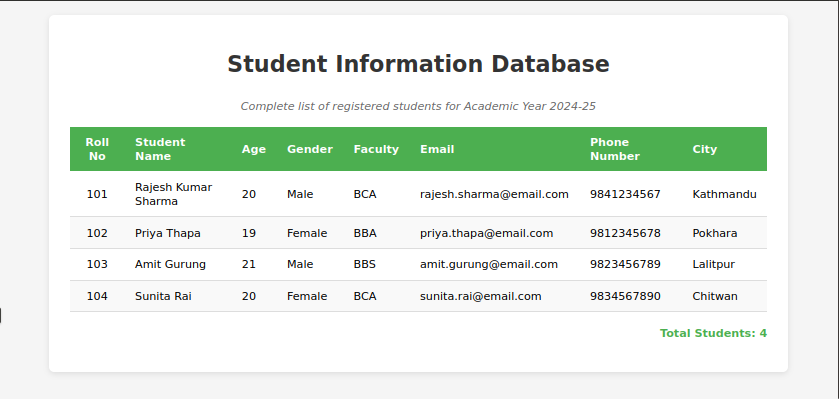
\includegraphics[width=0.8\textwidth]{9_screenshot.png}
    \caption{Student Information Table Output}
\end{figure}


\section{XML Examples}
This section includes XML structures for student registration and employee records, with an XSD for the employee XML.

\subsection{Student Registration XML}
Corrected XML for student registration data.

\lstset{language=XML}
\begin{lstlisting}
<?xml version="1.0" encoding="UTF-8"?>
<studentRegistration>
  <student>
    <rollNumber>101</rollNumber>
    <fullName>Rajesh Kumar Sharma</fullName>
    <address>123 Main St, Kathmandu</address>
    <phoneNumber>9841234567</phoneNumber>
    <gender>Male</gender>
    <dateOfBirth>2004-05-15</dateOfBirth>
    <subjects>
      <subject>Artificial Intelligence</subject>
      <subject>Database Administration</subject>
    </subjects>
    <faculty>BCA</faculty>
    <comments>Interested in AI research</comments>
  </student>
</studentRegistration>
\end{lstlisting}

\subsection{Employee Records XML}
XML for employee information with its schema.

\lstset{language=XML}
\begin{lstlisting}
<?xml version="1.0" encoding="UTF-8"?>
<employeeRecords>
    <employee>
        <name>Rajesh Kumar Sharma</name>
        <address>
            <temporary>123 Main St, Kathmandu</temporary>
            <permanent>456 Park Ave, Pokhara</permanent>
        </address>
        <phoneNumber>9841234567</phoneNumber>
        <age>30</age>
        <email>rajesh.sharma@company.com</email>
        <workLocation>Kathmandu Branch</workLocation>
    </employee>
</employeeRecords>
\end{lstlisting}

\lstset{language=XML}
\begin{lstlisting}
<?xml version="1.0" encoding="UTF-8"?>
<xs:schema xmlns:xs="http://www.w3.org/2001/XMLSchema">
    <xs:element name="employeeRecords">
        <xs:complexType>
            <xs:sequence>
                <xs:element name="employee" maxOccurs="unbounded">
                    <xs:complexType>
                        <xs:sequence>
                            <xs:element name="name" type="xs:string"/>
                            <xs:element name="address">
                                <xs:complexType>
                                    <xs:sequence>
                                        <xs:element name="temporary" type="xs:string"/>
                                        <xs:element name="permanent" type="xs:string"/>
                                    </xs:sequence>
                                </xs:complexType>
                            </xs:element>
                            <xs:element name="phoneNumber">
                                <xs:simpleType>
                                    <xs:restriction base="xs:string">
                                        <xs:pattern value="[0-9]{10}"/>
                                    </xs:restriction>
                                </xs:simpleType>
                            </xs:element>
                            <xs:element name="age">
                                <xs:simpleType>
                                    <xs:restriction base="xs:positiveInteger">
                                        <xs:minInclusive value="18"/>
                                        <xs:maxInclusive value="65"/>
                                    </xs:restriction>
                                </xs:simpleType>
                            </xs:element>
                            <xs:element name="email">
                                <xs:simpleType>
                                    <xs:restriction base="xs:string">
                                        <xs:pattern value="[a-zA-Z0-9._%+-]+@[a-zA-Z0-9.-]+\.[a-zA-Z]{2,}"/>
                                    </xs:restriction>
                                </xs:simpleType>
                            </xs:element>
                            <xs:element name="workLocation" type="xs:string"/>
                        </xs:sequence>
                    </xs:complexType>
                </xs:element>
            </xs:sequence>
        </xs:complexType>
    </xs:element>
</xs:schema>
\end{lstlisting}

\section{CRUD Operations with PHP}
The CRUD operations manage student data in a MySQL database "STUDENT" with table "BCA" (rollno, name, gender, phone). Each operation is presented with its complete code.

\subsection{Insertion Code}
The insertion operation uses an HTML form (\texttt{form.php}) and a PHP script (\texttt{insert.php}) with prepared statements for security.

\lstset{language=HTML}
\begin{lstlisting}
<!DOCTYPE html>
<html lang="en">
<head>
    <meta charset="UTF-8">
    <title>CRUD Operation</title>
    <style>
        * {
            box-sizing: border-box;
        }
        body {
            margin: 0;
            padding: 0;
            background: linear-gradient(to right, #74ebd5, #ACB6E5);
            font-family: 'Segoe UI', Tahoma, Geneva, Verdana, sans-serif;
            height: 100vh;
            display: flex;
            justify-content: center;
            align-items: center;
        }
        .form-container {
            background: #ffffff;
            padding: 30px 40px;
            border-radius: 15px;
            box-shadow: 0 10px 25px rgba(0, 0, 0, 0.15);
            width: 100%;
            max-width: 400px;
        }
        .form-container h2 {
            text-align: center;
            color: #333;
            margin-bottom: 20px;
        }
        label {
            font-weight: bold;
            margin-bottom: 5px;
            display: block;
            color: #333;
        }
        input[type="text"],
        input[type="number"],
        select {
            width: 100%;
            padding: 10px;
            margin-bottom: 20px;
            border: 2px solid #ccc;
            border-radius: 8px;
            transition: border 0.3s;
        }
        input[type="submit"] {
            width: 100%;
            padding: 12px;
            background-color: #4CAF50;
            border: none;
            border-radius: 8px;
            color: white;
            font-size: 16px;
            font-weight: bold;
            cursor: pointer;
            transition: background 0.3s;
        }
        .message {
            text-align: center;
            margin-bottom: 20px;
            font-weight: bold;
            color: green;
        }
    </style>
</head>
<body>
<div class="form-container">
    <h2>CRUD Operation</h2>
    <?php if (!empty($message)): ?>
        <div class="message <?= strpos($message, 'Error') !== false || strpos($message, 'required') !== false ? 'error' : '' ?>">
            <?= $message ?>
        </div>
    <?php endif; ?>
    <form method="post" action="./insert.php">
        <label for="rollno">Roll No:</label>
        <input type="number" name="rollno" id="rollno" required>
        <label for="name">Name:</label>
        <input type="text" name="name" id="name" required>
        <label for="gender">Gender:</label>
        <select name="gender" id="gender" required>
            <option value="">-- Select Gender --</option>
            <option value="Male">Male</option>
            <option value="Female">Female</option>
            <option value="Other">Other</option>
        </select>
        <label for="phone">Phone:</label>
        <input type="text" name="phone" id="phone" required>
        <input type="submit" value="Submit">
    </form>
    <a href="display.php" style="display: block; text-align: center; margin-top: 10px;">View All Records</a>
</div>
</body>
</html>
\end{lstlisting}

\lstset{language=PHP}
\begin{lstlisting}
<?php
// insert.php
$servername = "localhost";
$username = "root";
$password = "";
$database = "STUDENT";
$conn = new mysqli($servername, $username, $password, $database);
if ($conn->connect_error) {
    die("Connection failed: " . $conn->connect_error);
}
$stmt = $conn->prepare("INSERT INTO BCA (rollno, name, gender, phone) VALUES (?, ?, ?, ?)");
$stmt->bind_param("isss", $rollno, $name, $gender, $phone);
$rollno = $_POST['rollno'];
$name = $_POST['name'];
$gender = $_POST['gender'];
$phone = $_POST['phone'];
if ($stmt->execute()) {
    echo "Record inserted successfully!";
} else {
    echo "Error: " . $stmt->error;
}
$stmt->close();
$conn->close();
?>
\end{lstlisting}

\subsection{Deletion Code}
The deletion operation uses a PHP script (\texttt{delete.php}) to remove a record by roll number.

\lstset{language=PHP}
\begin{lstlisting}
<?php
// delete.php
$servername = "localhost";
$username = "root";
$password = "";
$database = "STUDENT";
$conn = new mysqli($servername, $username, $password, $database);
if ($conn->connect_error) {
    die("Connection failed: " . $conn->connect_error);
}
$rollno = $_GET['rollno'];
$stmt = $conn->prepare("DELETE FROM BCA WHERE rollno = ?");
$stmt->bind_param("i", $rollno);
if ($stmt->execute()) {
    header("Location: display.php");
} else {
    echo "Error deleting record: " . $stmt->error;
}
echo '<a href="display.php">Back to Records</a>';
$stmt->close();
$conn->close();
?>
\end{lstlisting}

\subsection{Update Code}
The update operation uses a PHP script (\texttt{update.php}) with an HTML form to modify existing records.

\lstset{language=PHP}
\begin{lstlisting}
<?php
// update.php
$servername = "localhost";
$username = "root";
$password = "";
$database = "STUDENT";
$conn = new mysqli($servername, $username, $password, $database);
if ($conn->connect_error) {
    die("Connection failed: " . $conn->connect_error);
}
$rollno = $_GET['rollno'];
if ($_SERVER['REQUEST_METHOD'] == 'POST') {
    $name = $_POST['name'];
    $gender = $_POST['gender'];
    $phone = $_POST['phone'];
    $stmt = $conn->prepare("UPDATE BCA SET name = ?, gender = ?, phone = ? WHERE rollno = ?");
    $stmt->bind_param("sssi", $name, $gender, $phone, $rollno);
    if ($stmt->execute()) {
        header("Location: display.php");
        exit();
    } else {
        echo "Error updating record: " . $stmt->error;
    }
    $stmt->close();
} else {
    $stmt = $conn->prepare("SELECT * FROM BCA WHERE rollno = ?");
    $stmt->bind_param("i", $rollno);
    $stmt->execute();
    $result = $stmt->get_result();
    $row = $result->fetch_assoc();
    $stmt->close();
}
?>
<!DOCTYPE html>
<html lang="en">
<head>
    <meta charset="UTF-8">
    <title>Update Record</title>
    <style>
        body {
            font-family: 'Segoe UI', Tahoma, Geneva, Verdana, sans-serif;
            margin: 20px;
        }
        h2 {
            text-align: center;
        }
        form {
            max-width: 400px;
            margin: 0 auto;
        }
        label {
            display: block;
            margin-bottom: 5px;
        }
        input, select {
            width: 100%;
            padding: 10px;
            margin-bottom: 10px;
            border: 1px solid #ccc;
            border-radius: 4px;
        }
        input[type="submit"] {
            background-color: #4CAF50;
            color: white;
            border: none;
            cursor: pointer;
        }
    </style>
</head>
<body>
    <h2>Update Record</h2>
    <form method="post">
        <label>Name:</label>
        <input type="text" name="name" value="<?= htmlspecialchars($row['name']) ?>" required>
        <label>Gender:</label>
        <select name="gender" required>
            <option value="Male" <?= $row['gender'] == 'Male' ? 'selected' : '' ?>>Male</option>
            <option value="Female" <?= $row['gender'] == 'Female' ? 'selected' : '' ?>>Female</option>
            <option value="Other" <?= $row['gender'] == 'Other' ? 'selected' : '' ?>>Other</option>
        </select>
        <label>Phone:</label>
        <input type="text" name="phone" value="<?= htmlspecialchars($row['phone']) ?>" required>
        <input type="submit" value="Update">
    </form>
</body>
</html>
<?php
$conn->close();
?>
\end{lstlisting}

\subsection{Display Code}
The display operation uses a PHP script (\texttt{display.php}) to show all records in a table.

\lstset{language=PHP}
\begin{lstlisting}
<?php
// display.php
error_reporting(E_ALL);
ini_set('display_errors', 1);
$servername = "localhost";
$username = "root";
$password = "";
$database = "STUDENT";
$conn = new mysqli($servername, $username, $password, $database);
if ($conn->connect_error) {
    die("Connection failed: " . $conn->connect_error);
}
echo "Connected successfully<br>";
$query = "SELECT * FROM BCA";
$data = mysqli_query($conn, $query);
if (!$data) {
    die("Query failed: " . mysqli_error($conn));
}
$total = mysqli_num_rows($data);
if ($total != 0) {
    echo "<table border='1' cellspacing='0' cellpadding='10'>";
    echo "<tr><th>rollno</th><th>name</th><th>gender</th><th>phone</th><th>Update</th><th>Delete</th></tr>";
    while ($result = mysqli_fetch_assoc($data)) {
        echo "<tr>";
        echo "<td>" . $result['rollno'] . "</td>";
        echo "<td>" . htmlspecialchars($result['name']) . "</td>";
        echo "<td>" . $result['gender'] . "</td>";
        echo "<td>" . $result['phone'] . "</td>";
        echo "<td><a href='update.php?rollno=" . $result['rollno'] . "'>Update</a></td>";
        echo "<td><a href='delete.php?rollno=" . $result['rollno'] . "' onclick='return confirm(\"Are you sure?\");'>Delete</a></td>";
        echo "</tr>";
    }
    echo "</table>";
} else {
    echo "No records found.";
}
$conn->close();
?>
<a href="form.php" style="display: block; text-align: center; margin-top: 10px;">Back to Form</a>
\end{lstlisting}


\subsection{CRUD Output}
The rendered output of the CRUD operations (e.g., form or display table) is shown below.

\begin{figure}[H]
    \centering
    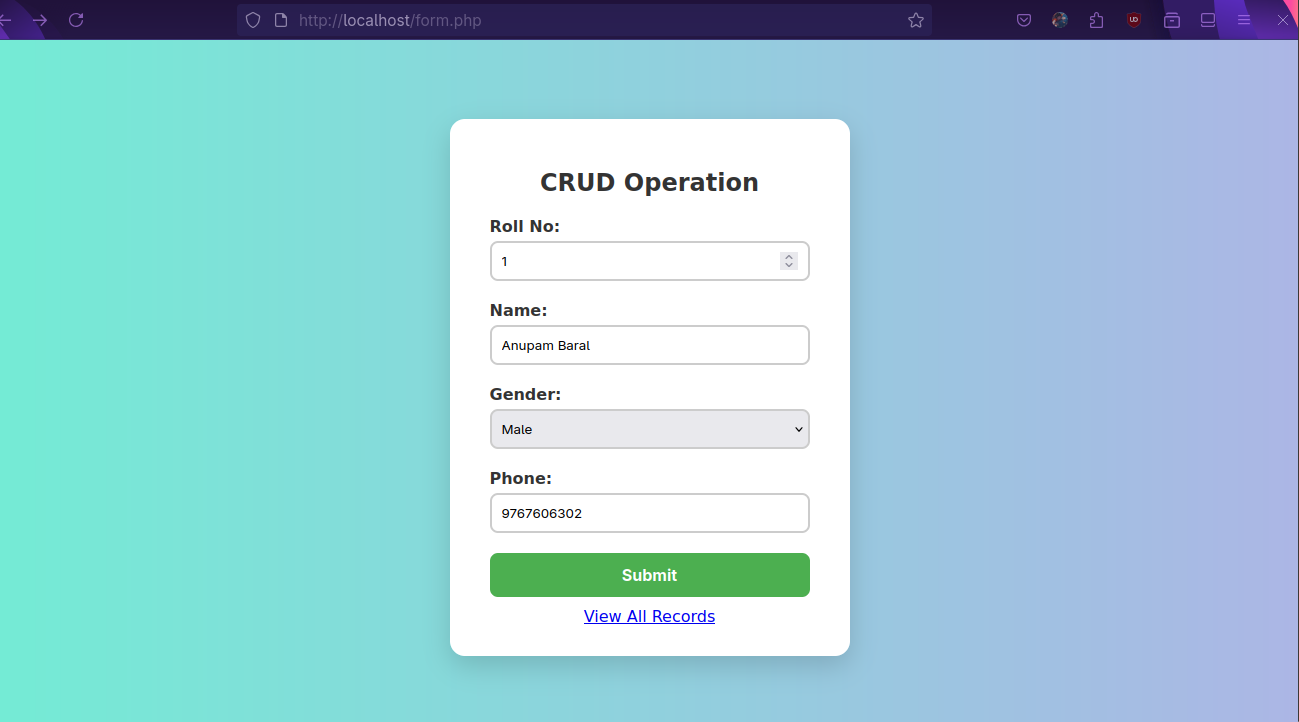
\includegraphics[width=0.8\textwidth]{5_screenshot.png}
    \caption{Form Output}
\end{figure}

\begin{figure}[H]
    \centering
    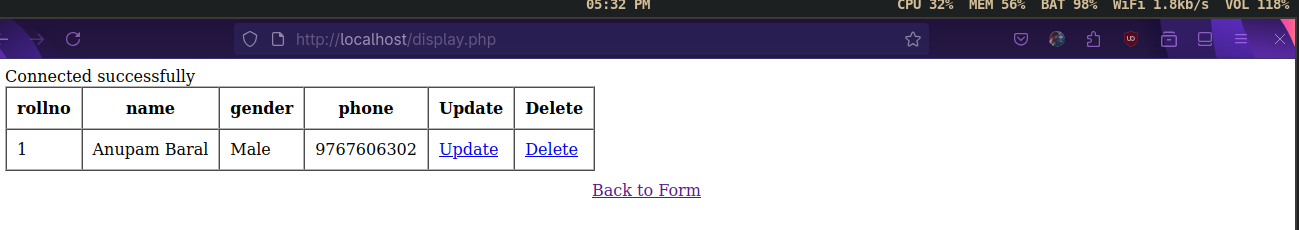
\includegraphics[width=0.8\textwidth]{6_screenshot.png}
    \caption{CRUD Operations Output(display.php)}
\end{figure}

\begin{figure}[H]
    \centering
    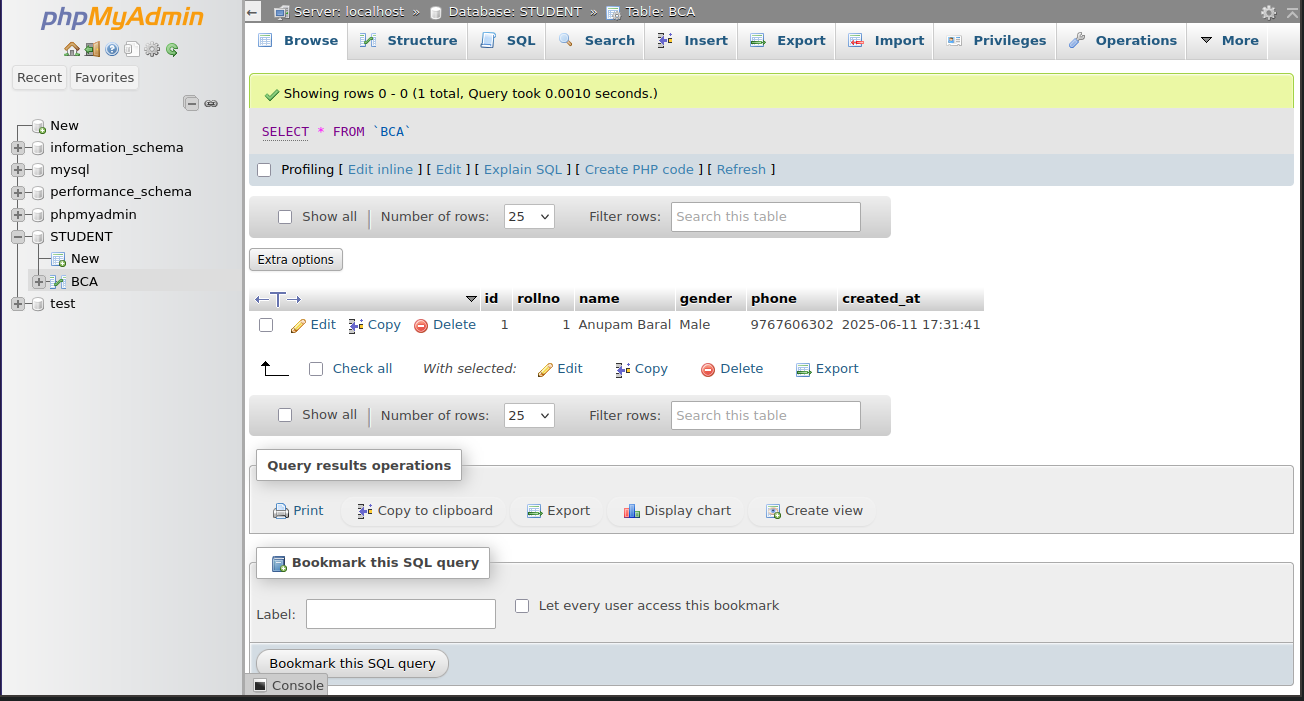
\includegraphics[width=0.95\textwidth, height=0.6\textheight]{7_screenshot.png}
    \caption{CRUD Operations Output(database)}
\end{figure}

\section{Conclusion}
This lab report presents a complete student registration system with HTML, CSS, PHP, MySQL, and XML, with all CRUD operations fully implemented, output images included, and formatted consistently.

\end{document}



\section{Conclusion}
This lab report presents a complete student registration system with HTML, CSS, PHP, MySQL, and XML, with all CRUD operations fully implemented, output images included, and formatted consistently.

\end{document}
